
\chapter{Estado del arte}
\label{cha:estado-del-arte}

\section{Introducción}
\label{sec:intro-sota}

\begin{FraseCelebre}
  \begin{Frase}
    Si buscas resultados distintos no hagas siempre lo mismo.
  \end{Frase}
  \begin{Fuente}
    Albert Einstein
  \end{Fuente}
\end{FraseCelebre}

\section{Técnicas utilizadas}
\label{sec:tecnicas-utilizadas}

\textcolor{red}{Aquí escribir todo lo que encuentre sobre artículos donde detecten objetos abandonados mediante el uso de aplicaciones de videovigilancia}

\subsection{Segmentación de objetos en primer plano}
\label{subsec:tecnicas-segmentacion-obj-primer-plano}

\cite{BOUWMANS201431} y \cite{YAZDI2018157}

\newpage

\subsection{Detección de objetos estacionarios}
\label{subsec:tecnicas-deteccion-obj-estacionarios}

\cite{5279450} y \cite{CUEVAS201641}

\newpage

\subsection{Detección de personas}
\label{subsec:tecnicas-deteccion-personas}

\cite{4657363}, y \cite{https://doi.org/10.1049/iet-cvi.2014.0148}

\newpage

\subsection{Reconocimiento del comportamiento}
\label{subsec:tecnicas-reconocimiento-comportamiento}

\cite{vishwakarma2012}, \cite{borges2013}, \cite{popoola2012} y \cite{BENMABROUK2018480}

\newpage

\section{Redes neuronales convolucionales}

\textcolor{red}{Mirar este artículo como introductorio \url{https://arxiv.org/pdf/2011.12960.pdf}}

\newpage

\section{Algoritmos de detección de objetos}
\label{sec:tecnicas-utilizadas-detection}

\subsection{Fast R-CNN}
\label{subsec:fast-rcnn}

Fast \gls{r-cnn} es una red blablabla

\newpage

\subsection{Faster R-CNN}
\label{subsec:faster-rcnn}

\newpage

\subsection{SSD: Single Shot MultiBox Detector}
\label{subsec:ssd}

\newpage

\subsection{EfficientDet}
\label{subsec:efficientdet}

\newpage

\subsection{YOLO: You Only Look Once}
\label{subsec:yolo}

Presentar YOLO y hacer énfasis en YOLOv4

\newpage

\section{Algoritmos de seguimiento de objetos}
\label{sec:tecnicas-utilizadas-tracking}

\subsection{Filtro de Kalman}
\label{subsec:kalman-filter}

En azul y naranja las detecciones, deepsort cuadros delimitadores blancos.

Explicar filtro de Kalman

\textcolor{red}{Meter imágenes de ejemplo de se visualice bien el cuadro delimitador de detección y el de seguimiento}

\newpage

\subsection{Algoritmo húngaro}
\label{subsec:hungarian-algorithm}

Explicar algoritmo húngaro.

\newpage

\subsection{DeepSORT}
\label{subsec:deepsort}

Explicar que se trata de un algoritmo que combina El filtro de Kalman con el algoritmo húngaro.

\begin{figure}[ht]
\centering
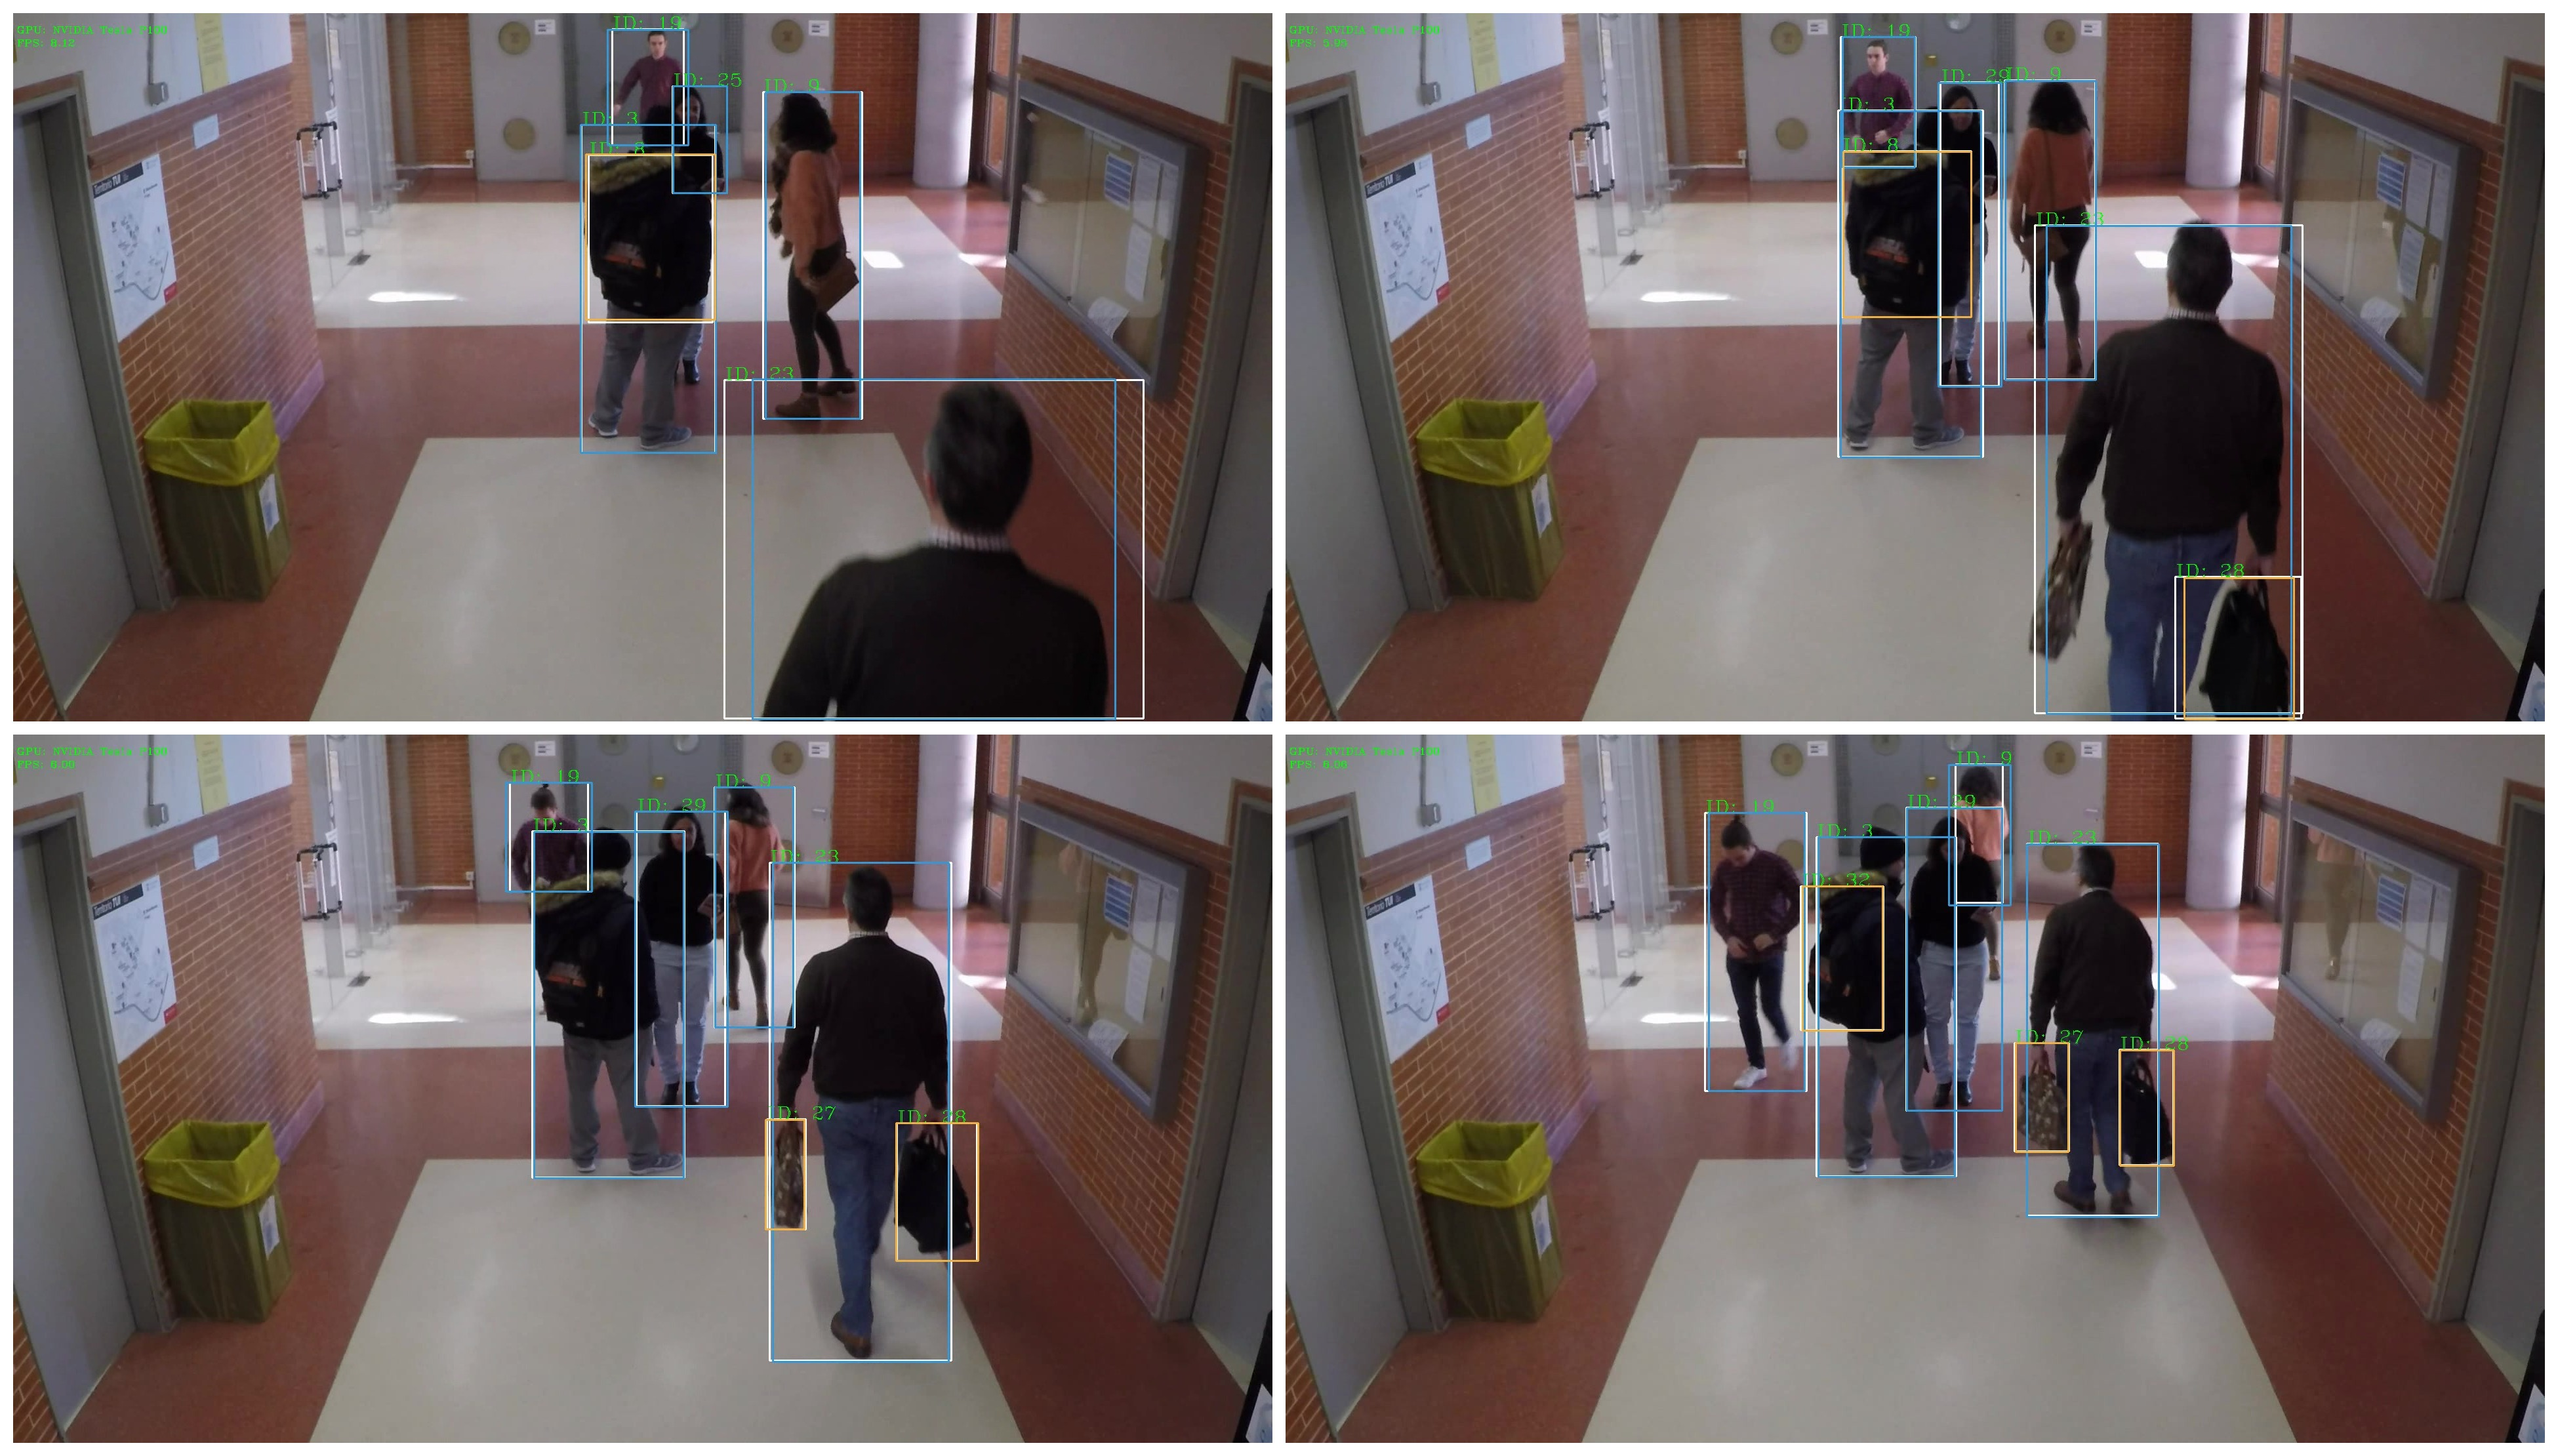
\includegraphics[width=1\textwidth]{img/chapters/algoritmos/deepsort-example.png}
\caption{\label{fig:tracking-example}Funcionamiento de Deepsort}
\end{figure}

\newpage

\section{Conclusiones}
\label{sec:conclu-sota}